\chapter{Projeto Conceitual do Produto}

\section{Características gerais}

O produto consiste em um robô autônomo que resolve labirintos. O robô pode resolver labirintos de distintos tamanhos e diversas configurações, além de transmitir em tempo real dados de consumo energético, velocidade e um mapa do labirinto. Essas informações são provenientes de sensores de distância infravermelhos e ultrasônicos, que enviam dados a um microcontrolador Raspberry Pi Pico, que os interpreta e calcula a distância do robô em relação as paredes. Além disso, para dados de consumo energético, o micromouse conta com sensores de tensão e corrente analógicos, que oferecem dados precisos do tempo de bateria restante. O Software é baseado nos projetos mais utilizados em competições de micromouse e foi projetado para resolver de maneira consistente cada problema apresentado. Por fim, o robô foi feito para ser compacto e robusto, capaz de navegar por entre os corredores apertados de maneira ágil e resistente a pequenos choques mecânicos em casos de acidentes.
\begin{landscape}
    \begin{figure}[htbp]
    \centering
    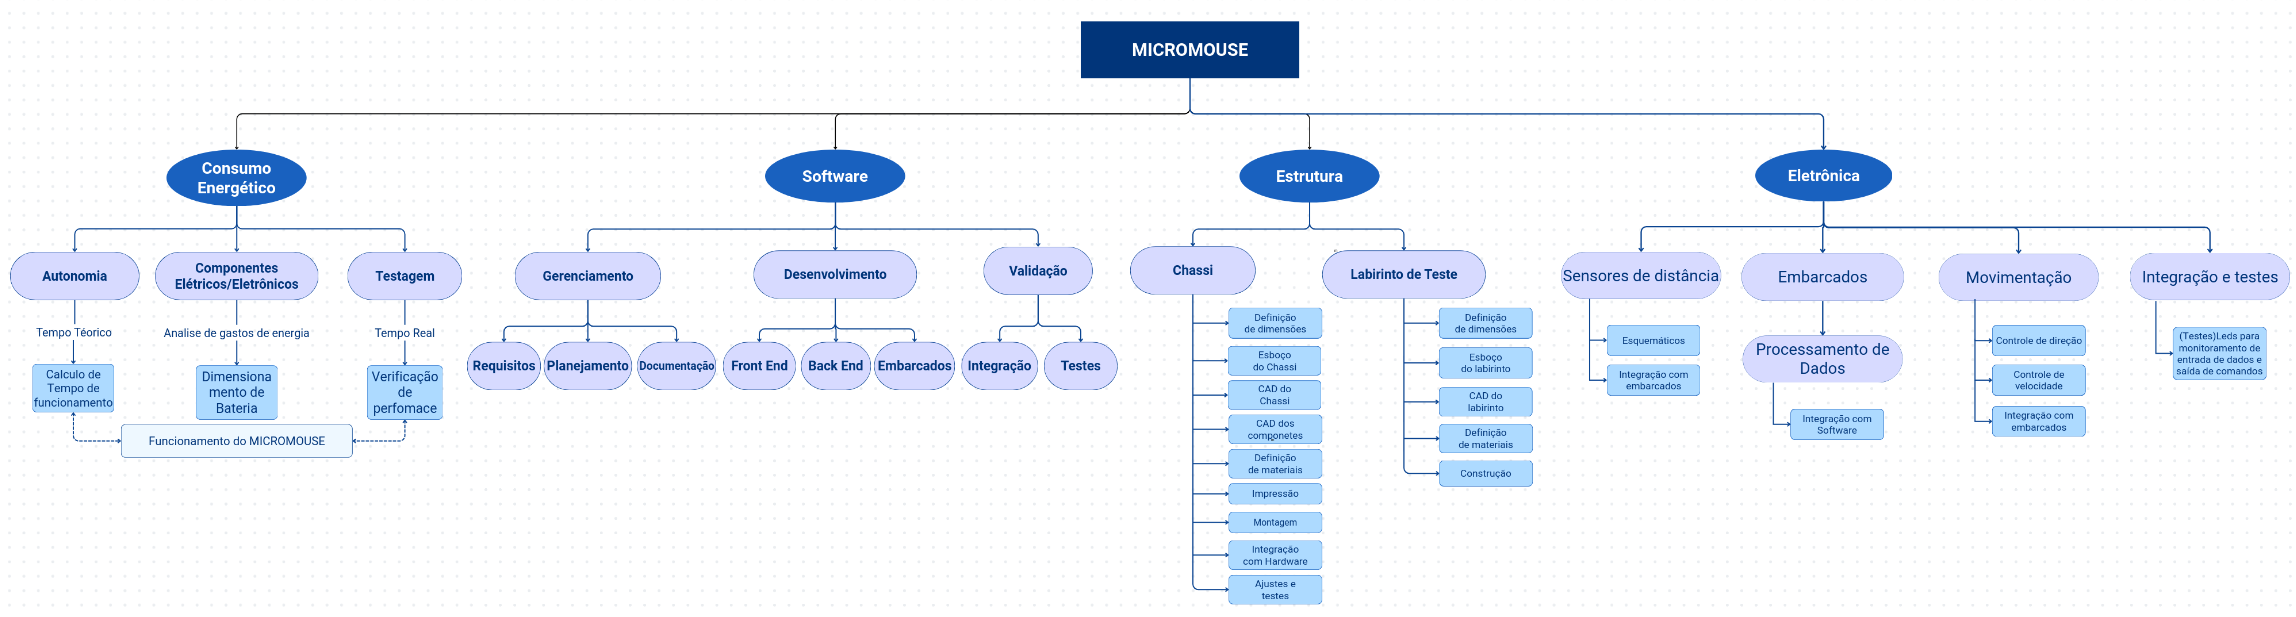
\includegraphics[width=1\linewidth]{figuras/eap_pi1_correta.png}
    \caption{Estrutura Analítica do Projeto (EAP)}
    \label{fig:EAP}
\end{figure}
\end{landscape}




% \textcolor{red}{Apresentar e explicar a Estrutura Analítica do Projeto (EAP), tomando cuidado com a legibilidade da imagem. Se necessário, coloque a EAP dentro do comando ``\textsf{\textbackslash begin\{landscape\} \textbackslash end\{landscape\}}'' para que ela seja apresentada em uma página deitada.}

\section{Estrutura}

A estrutura mecânica do micromouse foi desenhada em {\itshape Computer-Aided Design (CAD)} no software Catia V5, com o objetivo de acomodar todos os componentes eletrônicos, motores e baterias em um volume compatível com as dimensões máximas das células dos labirintos propostos (18\,cm de comprimento e 18\,cm de largura).

O micromouse possui dois níveis/andares para comportar confortavelmente as partes necessárias. A ideia inicial era que o chassi fosse composto por apenas um nível com todos os componentes, mas adicioná-los todos juntos faria com que ficassem apertados ou que as dimensões do robô ficassem grandes, e não queriamos comprometer a mobilidade, arriscando curvas apertadas. Logo, decidiu-se fazê-lo com dois níveis de chassi, com espessura de 4 mm cada. 

No projeto final teórico do micromouse, no primeiro nível encontram-se os dois motores N20 com encoders de 6V cada, as rodas, a principal placa de componentes eletrônicos e a esfera deslizante da frente. No segundo nível, estão as duas baterias de 3,7 V e mais uma pequena placa de componentes eletrônicos. Foram também modeladas abraçadeiras em U para a fixação dos motores, que possuem as dimensões dos componentes que aportam, presas ao chassi com 2 parafusos M2 (2 mm de diâmetro), também acompanhados dos insertos de latão.

A primeira versão da estrutura do micromouse, que foi enviada em ambos os pontos de controle 1 e 2 do projeto, possuia abraçadeiras em U também para as baterias no nível superior. O uso delas foi descartado na versão final, pois ambos os chassis inferior e superior foram remodelados para diminuir as dimensões horizontais do robô e oferecer maior margem de segurança nas curvas. Atualmente, as baterias ficam dentro de uma berço de um 5,5 cm de altura e 2 mm de espessura de parede, que possui uma abertura lateral para a passagem dos fios que vão para o chassi inferior.

Porém, em função de problemas graves de componentes eletrônicos na última semana do projeto, para a versão final real, retirou-se as placas perfuradas de fibra de vidro e substituiu-se por um protoboard encaixada no primeiro andar, que, infelizmente, ultrapassa as medidas horizontais previstas para o micromouse, porém, permitia que ele continuasse a andar.

A esfera deslizante e as abraçadeiras do motor são fixadas no chassi por parafusos M2 (2 mm de diâmetro). Já os espaçadores de nível são peças de nylon hexagonais com círculo circunscrito de diâmetro 5,6 mm e rosca de parafusos M3 (3 mm de diâmetro), tendo ambos as roscas fêmea e macho, que serão complementadas por um parafuso M3 no chassi inferior e um inserto de latão no chassi superior. Os insertos de latão utilizados são peças serrilhadas termofixáveis que possuem rosca interna para facilitar a parafusação no chassi impresso em filamento. Eles foram instalados em todos os locais de parafusos, com o leve aquecimento dos furos do chassi com um ferro de solda e a inserção. Para isso, é também necessário aumentar o diâmetro dos furos a serem impressos, dado que a peça possui espessura além do diâmetro da rosca interna, assim transformando os furos de 2 mm (parafuso M2) em 3,2 mm de diâmetro e os furos de 3 mm (parafuso M3) em 4,7 mm de diâmetro.

A Figura \ref{fig:cad_iso} apresenta a vista isométrica da versão final ideal do assembly do micromouse, na qual é possível observar o berço das baterias de 3,7 V no segundo nível e a separação entre os níveis.

\vspace{0.4in}

\begin{figure}[H]
    \centering
    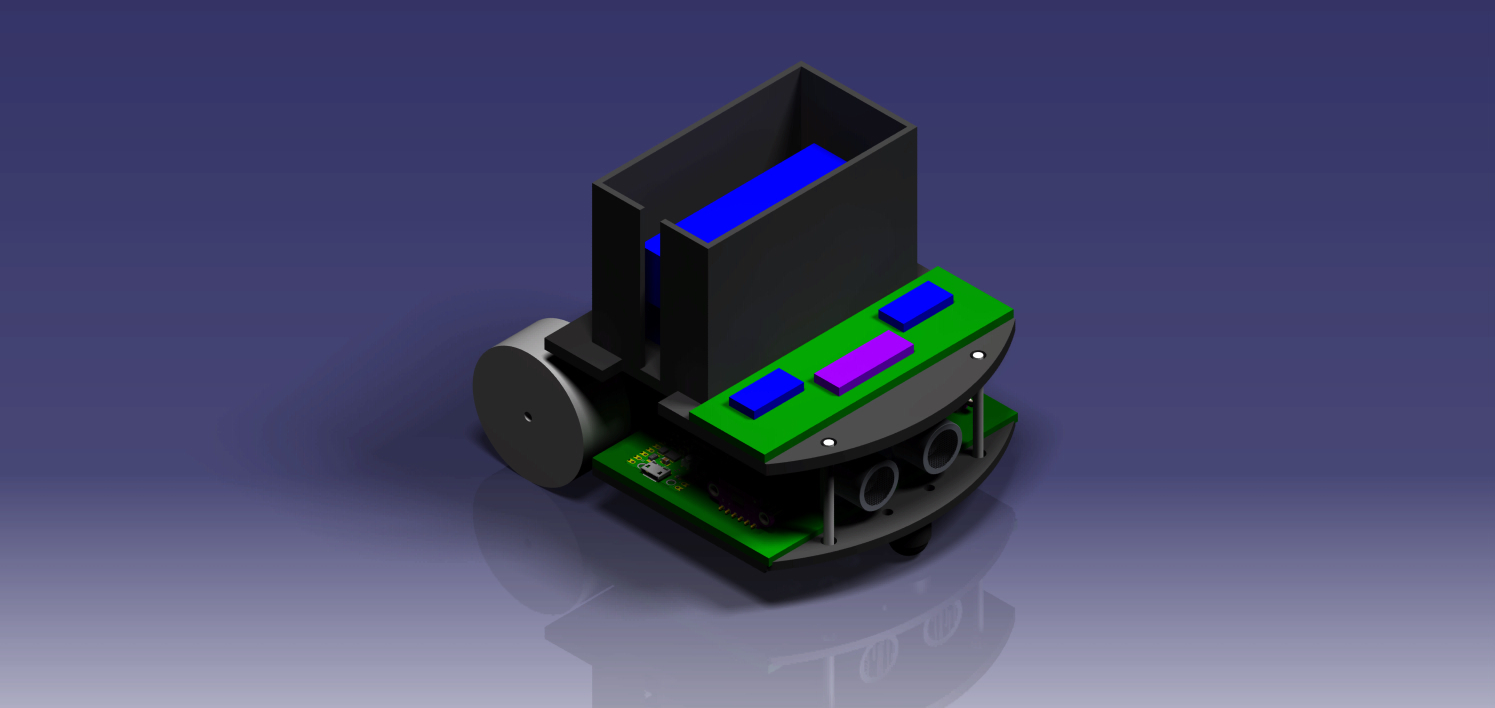
\includegraphics[width=0.85\linewidth]{figuras/render_final_iso.jpg}
    \caption{Vista isométrica da versão final do CAD do assembly do micromouse.}
    \label{fig:cad_iso}
\end{figure}

\vspace{0.15in}

A Figura \ref{fig:cad_superior} mostra a vista superior do primeiro nível do micromouse, na qual são identificados a placa de componentes eletrônicos principal. Os sensores frontais estão posicionados de forma a cobrir as três direções de interesse para a navegação: frente, esquerda e direita, conforme requerido pelo algoritmo de flood-fill descrito na Seção 6.5. Além disso, pode-se identificar os dois motores N20, fixados por abraçadeiras em U e as rodas em seus respectivos eixos.

\vspace{0.15in}

\begin{figure}[H]
    \centering
    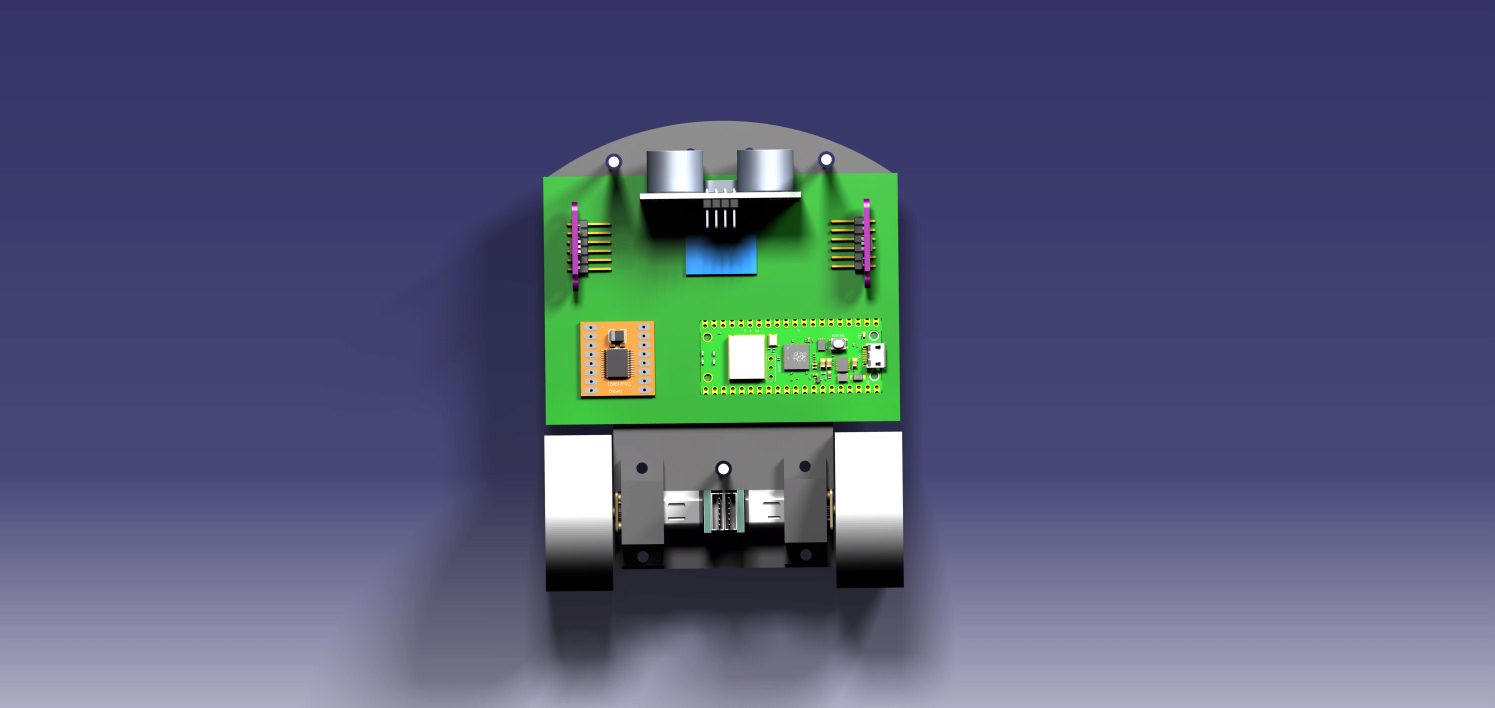
\includegraphics[width=0.85\linewidth]{figuras/render_final_superior1andar.jpg}
    \caption{Vista superior da versão final do CAD do primeiro nível do micromouse.}
    \label{fig:cad_superior}
\end{figure}

\vspace{0.13in}

O chassi e as abraçadeiras em U foram feitos com impressão 3D em filamento PETG, escolhido pelos benefícios proporcionados pela técnica, como a facilidade e agilidade de fabricação, a adaptação à geometrias personalizadas sem desperdício de material, assim como leveza, baixo custo e boa compatibilidade do material com as necessidades do projeto, como suportar cargas leves e resistir a perfurações. Já a placa de componentes eletrônicos foi feita em placa pré perfurada de fibra de vidro. Com os imprevistos que ocorreram no final do projeto, os componentes foram passados para a protoboard adaptada.

A Figura \ref{fig:cad_drafting} mostra as cotas e dimensões estabelecidas para a versão final teórica do micromouse, assim como a indicação da posição de cada componente.

\begin{landscape} 
\begin{figure}[H]
    \centering
    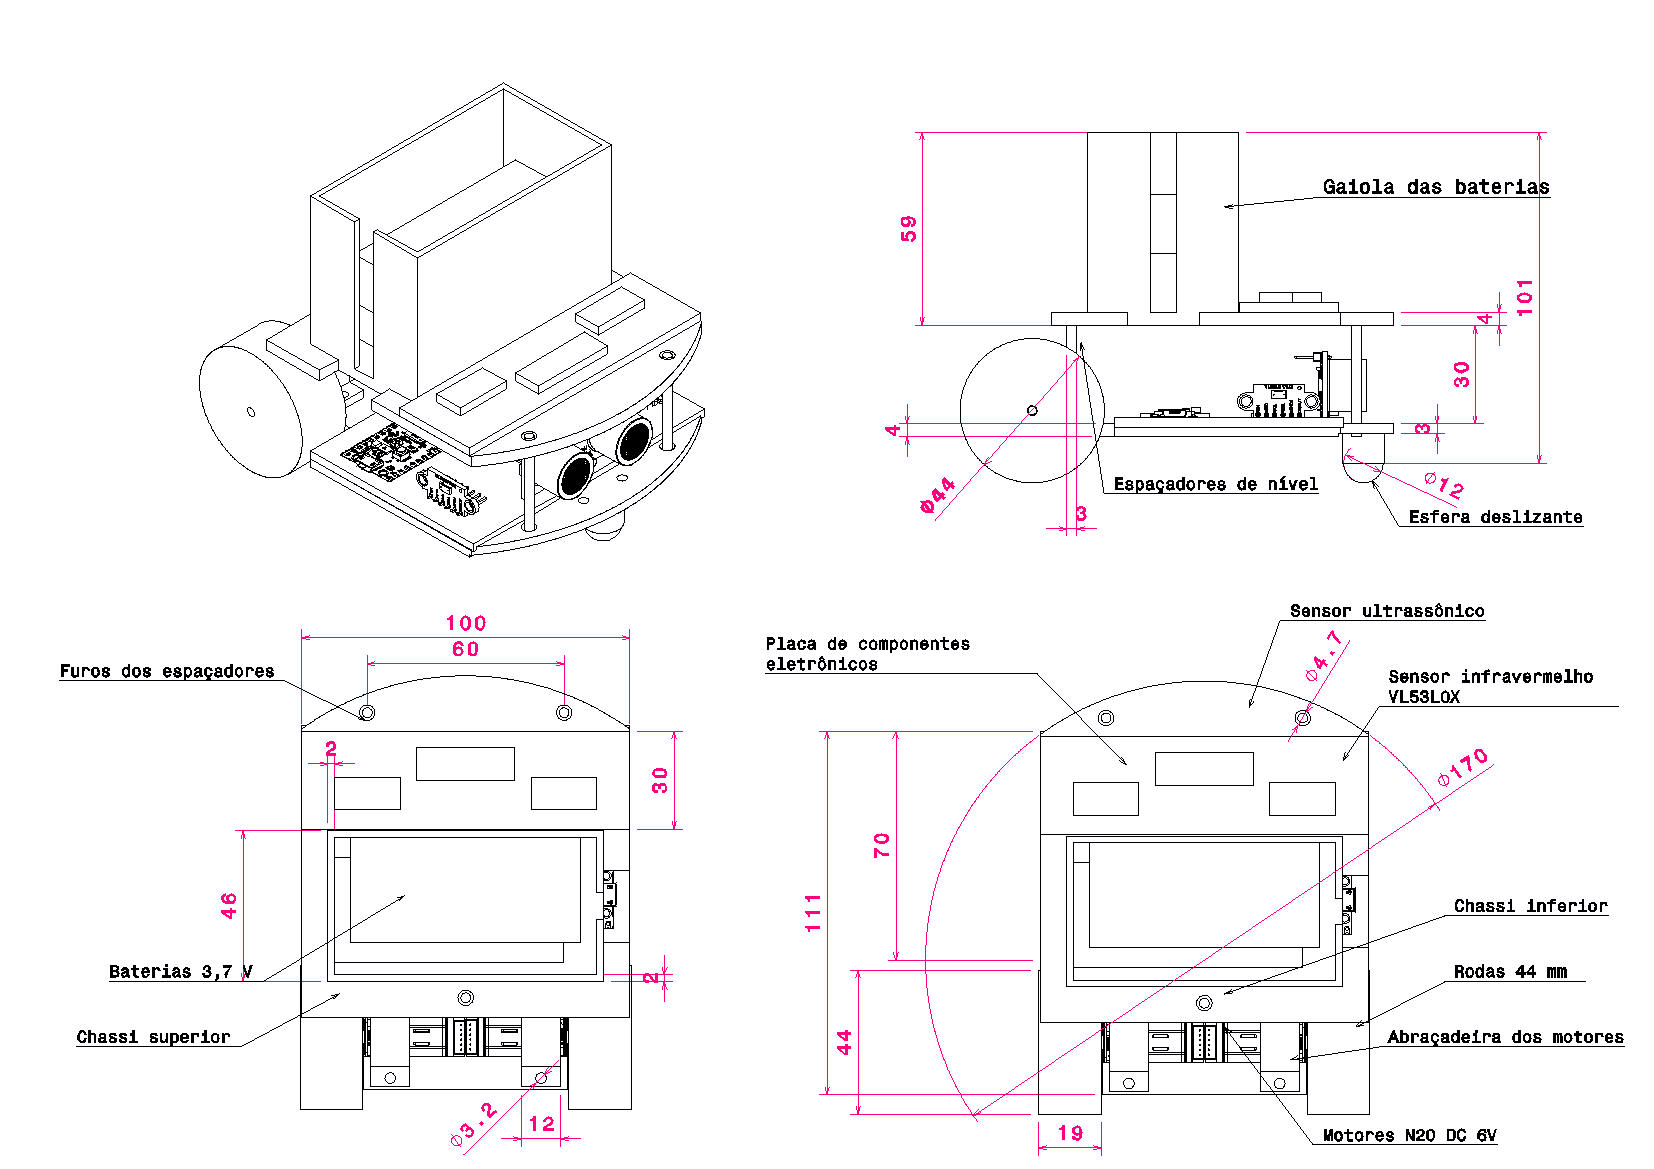
\includegraphics[width=0.86\linewidth]{figuras/mouse_drafting_2.jpg}
    \caption{Drafting da versão final do CAD do assembly do micromouse.}
    \label{fig:cad_drafting}
\end{figure}
\end{landscape}

\section{Descrição de \textit{hardware}}

%textcolor{red}{A descrição de \textit{hardware} no documento deve permitir que outras pessoas repliquem o produto proposto neste documento. Para isso, deve-se explicar de forma textual os principais sub-sistemas e as escolhas de projeto, além de indicar:}

O diagrama de blocos é uma ferramenta importante dentro de nosso projeto de engenharia, através do qual vamos apresentar uma visão geral da estrutura e interconexão entre os sistemas dos componentes eletrônicos de nosso modelo de projeto. O Diagrama foi realizado no site Lucidchart. Este é definido por blocos, cada um deles representando uma parte específica do processo ou sistema, os quais estarão conectados por meio de setas que se encarregam de mostrar de forma clara a direção do fluxo de dados e as linhas de alimentação com cores diferentes para maior compreensão.


\begin{figure}[H]
    \centering
    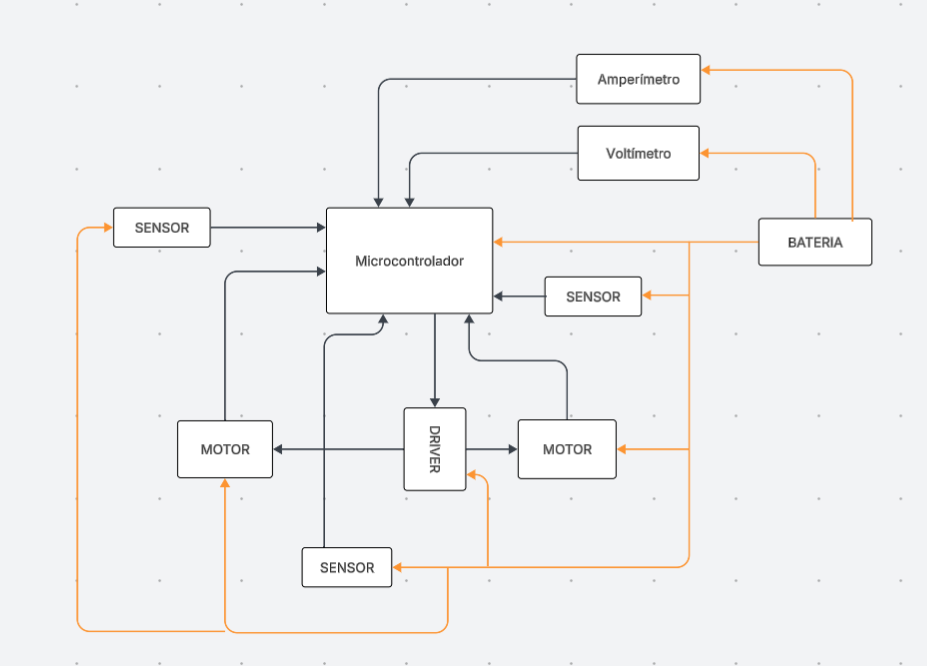
\includegraphics[width=1\linewidth]{figuras/Diagrama_de_blocos.png}
    \caption{Diagrama de blocos com os principais sistemas do robô.}
    \label{fig:diagrama_blocos}
\end{figure}

\par O esquemático, neste contexto, apresenta uma representação lógica e organizada dos componentes eletrônicos do projeto e da forma como eles se interligam por meio de símbolos universais. O foco é mostrar o fluxo de sinais e a conectividade elétrica entre os elementos do mapa lógico, fornecendo uma visão clara da arquitetura do hardware utilizado.

\begin{figure}[H]
    \centering
    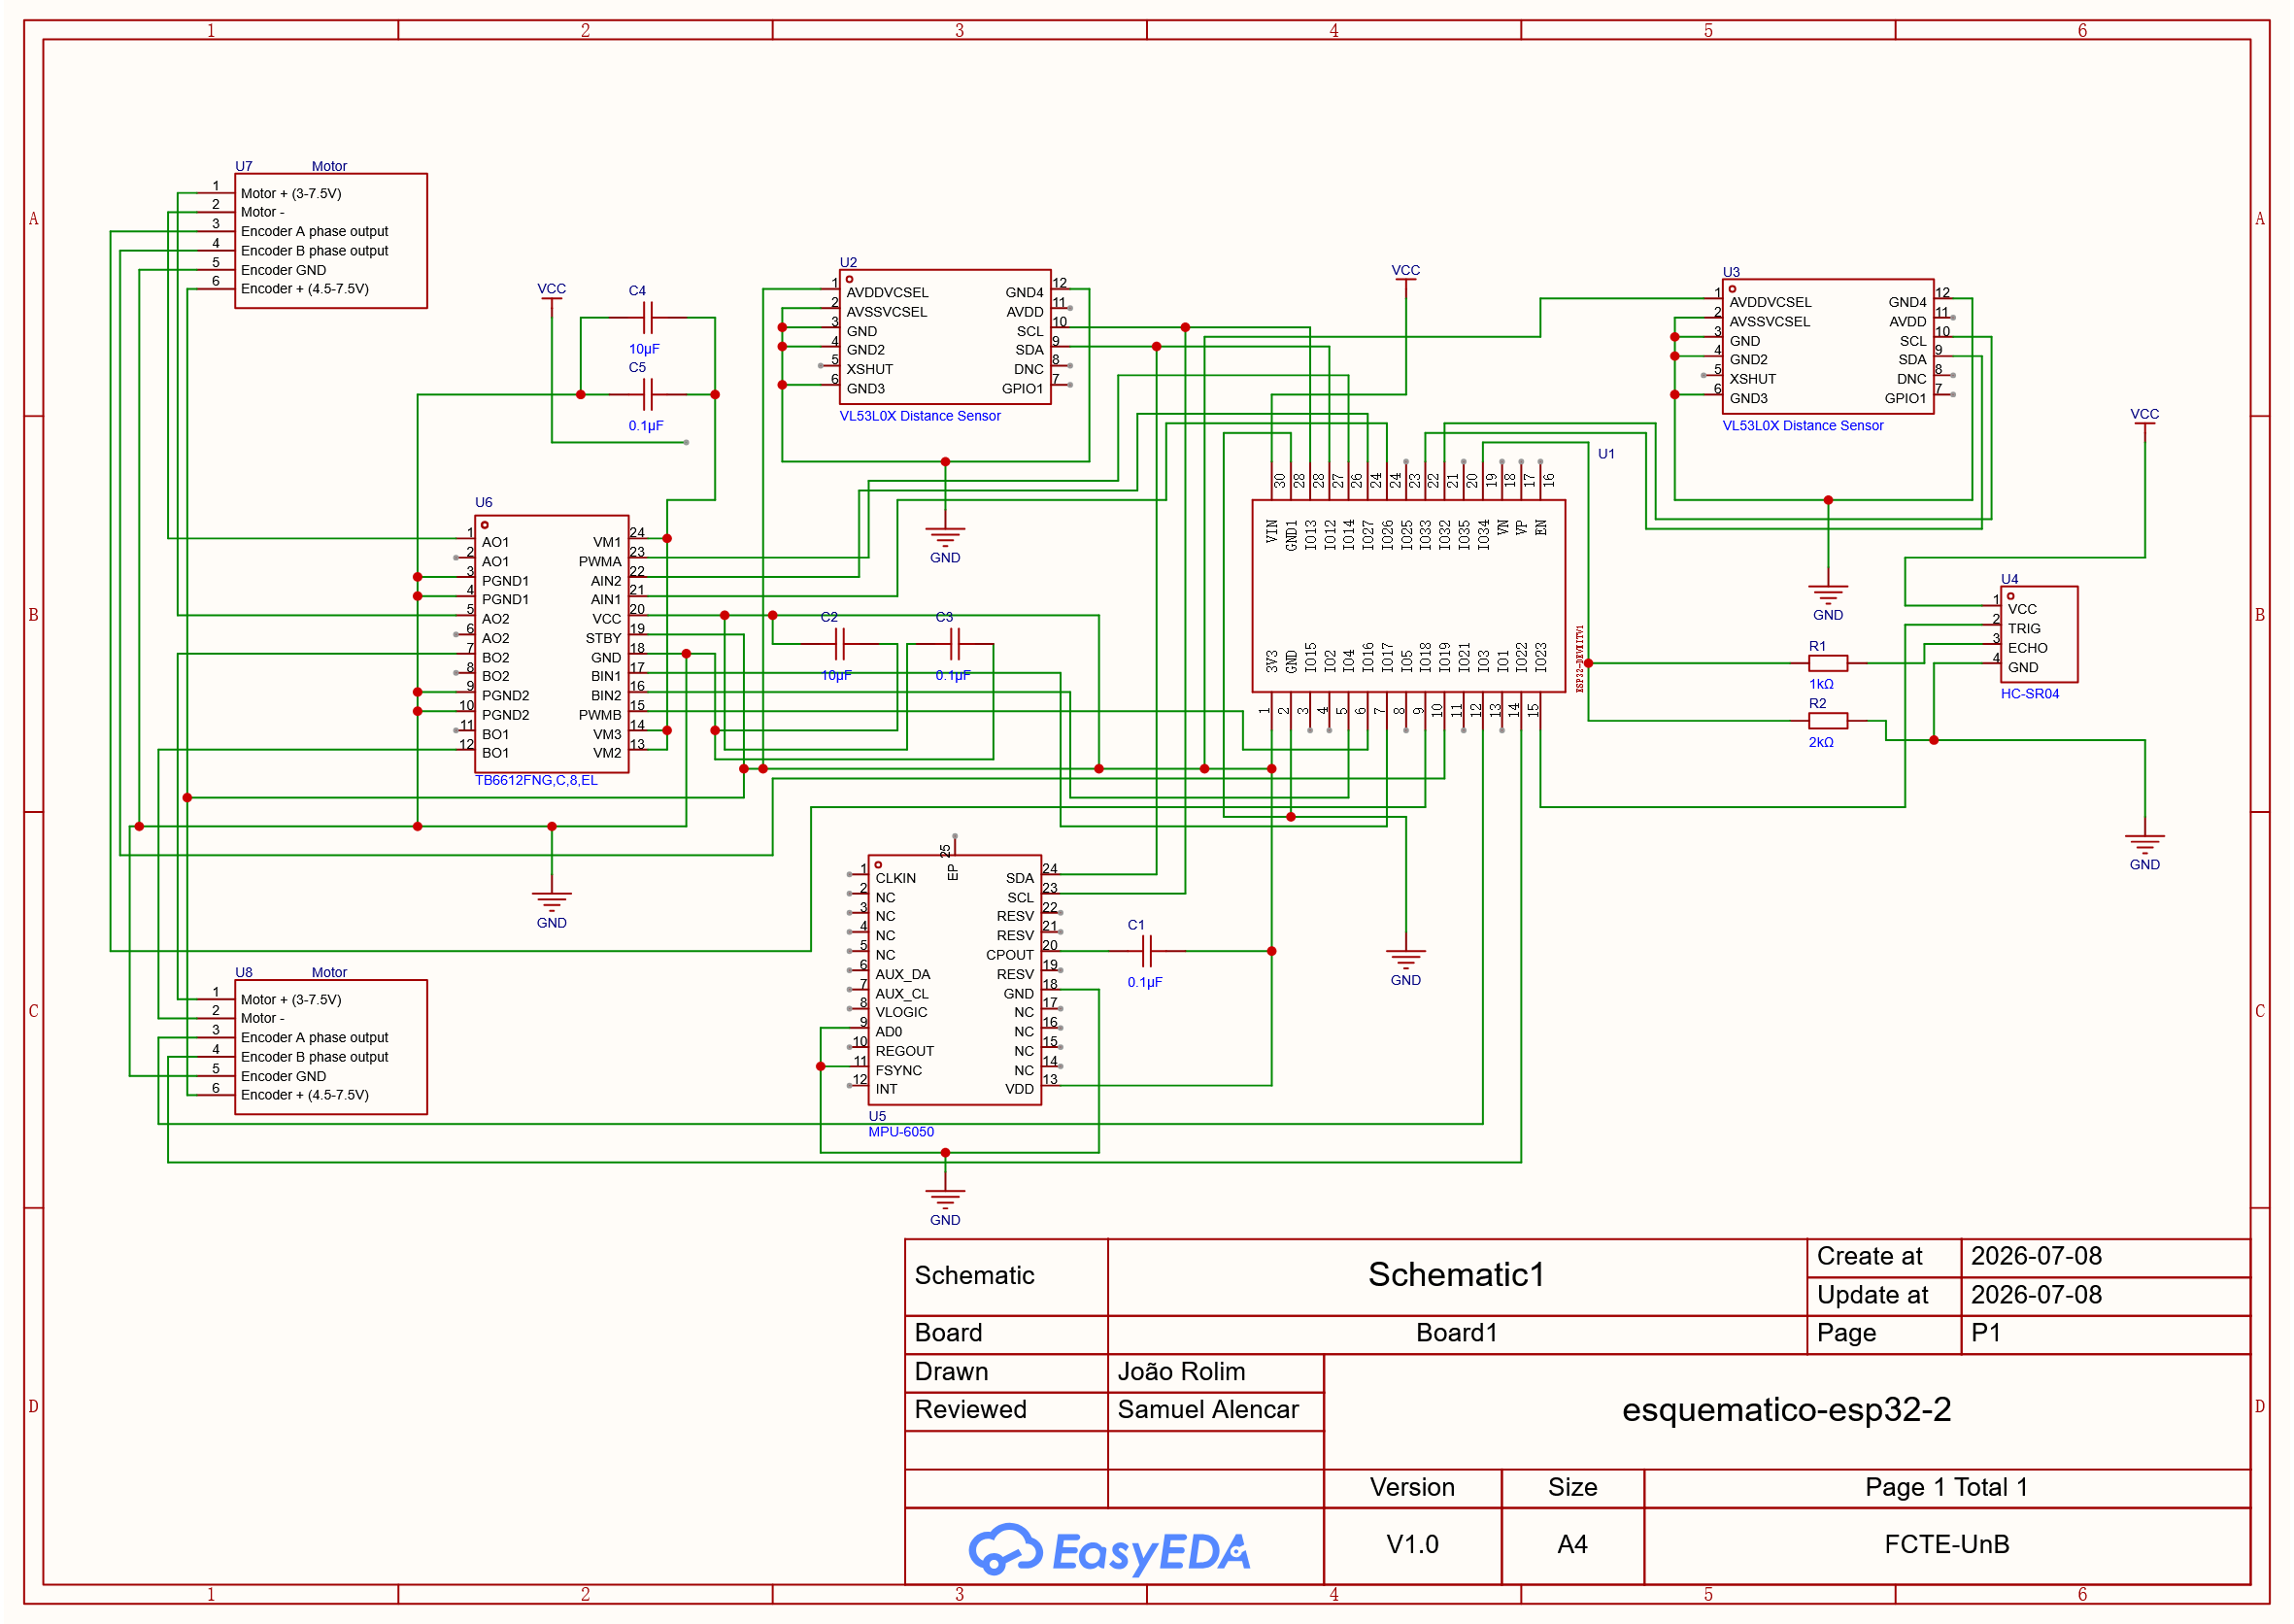
\includegraphics[width=1\linewidth]{figuras/SCH_Schematic1_1-P1_2026-07-08.png}
    \caption{Esquemático das conexões elétricas entre os componentes do robô.}
    \label{fig:esquematico_novo}
\end{figure}

\section{Análise de consumo energético}

A primeira etapa do dimensionamento energético do Micro Mouse consistiu na 
definição das características eletrônicas do sistema, com base nos equipamentos 
propostos e listados na Tabela \ref{tab:subsistemas_eletricos}. Por meio de um balanço de cargas, foi possível 
estimar o consumo total do circuito e, a partir disso, selecionar uma bateria 
adequada às demandas da aplicação.

\begin{table}[H]
    \centering
    \caption{Identificação dos Subsistemas Elétricos}
    \label{tab:subsistemas_eletricos}
    \resizebox{0.95\textwidth}{!}{%
    \begin{tabular}{|p{2.5cm}|p{4cm}|c|c|c|}
\hline
\textbf{Item} & \textbf{Especificação} & \textbf{Tensão (V)} & \textbf{Corrente (mA)} & \textbf{Energia consumida (J)} \\ \hline

Sensor & VL53LOX & 2,8 & 150 & 7560 \\ \hline
Sensor & HCSRO4 & 5 & 2 & 180 \\ \hline
Sensor & TB6612FNG & 2,7 & 1200 & 34992 \\ \hline
Sensor & MPU-6050 & 3,3 & 3,6 & 42,768 \\ \hline
Motor & GA12-N20 & 3 & 100 & 2160 \\ \hline
Placa & Placa de Fenolite & 0 & 0 & 0 \\ \hline
Placa & Perclorato de Ferro & 0 & 0 & 0 \\ \hline
Placa & Ferro de Solda & 0 & 0 & 0 \\ \hline
Controlador & Raspberry Pi Pico W & - & - & 7,2 \\ \hline
LED & --- & 2 & 20 & 0,04 \\ \hline
    \end{tabular}%
    }
\end{table}

Para o acionamento dos motores de tração modelo GA12-N20, foi adotado o driver 
de motor TB6612FNG, componente amplamente utilizado em sistemas de robótica 
embarcada por suportar a corrente demandada e permitir o controle bidirecional 
de velocidade e sentido de rotação de forma simples e eficiente. Em comparação 
com drivers convencionais baseados em transistores bipolares, o TB6612FNG 
apresenta menor dissipação de calor, maior eficiência energética e dimensões 
reduzidas, características especialmente vantajosas em robôs móveis de pequeno 
porte \cite{misra2018}.

Como sensores de proximidade, foram incorporadas duas tecnologias distintas: o 
sensor de distância por tempo de voo VL53L0X e o sensor ultrassônico HCSR04. 
Essa abordagem dual confere flexibilidade ao sistema, permitindo que equipes 
futuras avaliem e selecionem a tecnologia mais adequada durante os testes e o 
desenvolvimento dos algoritmos de navegação. Os sensores foram dispostos nas 
três direções principais — frontal e laterais —, ampliando o campo de percepção 
do robô e possibilitando uma navegação mais precisa no labirinto (MISRA; ADLER, 
2018). Para o monitoramento da orientação e movimentação do robô, foi 
incorporado o sensor inercial MPU-6050, que integra acelerômetro e giroscópio de 
três eixos, permitindo a estimativa de posição e o auxílio no controle de trajetória 
durante a navegação \cite{feitosa2025}.

Para o monitoramento do sistema elétrico em tempo real, foram integrados um 
módulo sensor de corrente com capacidade de até 5 A e um módulo sensor de 
tensão com faixa de operação de 0 a 25 V. Esses sensores permitem acompanhar 
continuamente o estado da bateria e o consumo dos componentes durante a 
operação, contribuindo para a segurança do sistema e para a análise de 
desempenho energético \cite{rashid2014}.

O microcontrolador selecionado foi o Raspberry Pi Pico W, em razão de seu bom 
desempenho de processamento, ampla documentação disponível na literatura e, 
principalmente, pela conectividade nativa Wi-Fi \cite{feitosa2025}.

Com os componentes e seus respectivos consumos devidamente levantados, 
conforme apresentado na Tabela \ref{tab:subsistemas_eletricos}, o consumo total estimado do sistema é de 
aproximadamente 1,8 A em operação nominal. Esse valor é dominado pelo driver 
de motor TB6612FNG, responsável por cerca de 65\% do consumo total do circuito. 
Procedeu-se então ao dimensionamento da fonte de energia, calculando a 
capacidade necessária da bateria com base no consumo estimado de cada 
componente ao longo do tempo de operação esperado.

Sobre esse valor, foi aplicada uma margem de segurança de 50\%, prática 
recomendada em projetos de sistemas embarcados \cite{rashid2014}, justificada por 
três fatores principais neste projeto. O primeiro é o comportamento dos motores de 
corrente contínua GA12-N20, que podem demandar correntes de partida e de 
manobra de três a cinco vezes superiores à corrente nominal, elevando o consumo 
total do sistema para valores próximos de 3,5 A a 4 A em situações de aceleração 
brusca ou mudança de direção no labirinto. O segundo fator é a degradação natural 
das células LiPo ao longo dos ciclos de carga e descarga: após 20 a 30 ciclos, a 
capacidade real da bateria pode ser reduzida para 85 a 90\% do valor nominal, 
comprometendo a autonomia do sistema caso não haja uma reserva energética 
adequada. O terceiro fator são as eventuais imprecisões nas especificações 
nominais dos componentes, que podem diferir do consumo real em condições de 
operação \cite{rashid2014}.

Com base nesse critério, optou-se por duas baterias de polímero de lítio (LiPo) de 
3,7 V e capacidade de 3000 mAh cada, conectadas em série, resultando em uma 
tensão nominal de 7,4 V e capacidade útil efetiva de 2000 mAh após a aplicação da 
margem de segurança. Essa configuração proporciona uma autonomia estimada 
de operação contínua superior a 60 minutos — valor significativamente acima do 
tempo médio de uma rodada na competição Micro Mouse —, o que confere ao 
sistema confiabilidade energética adequada para a aplicação proposta. A escolha 
pela tecnologia LiPo justifica-se pela sua elevada densidade energética, baixo peso 
e compatibilidade com sistemas embarcados de pequeno porte \cite{feitosa2025}.

Após a montagem física do protótipo, deverão ser realizados testes experimentais 
para validação do modelo energético teórico adotado. Durante esses ensaios, 
serão monitorados parâmetros como corrente média consumida, temperatura dos 
reguladores de tensão, estabilidade do sistema e autonomia prática da bateria. Os 
resultados obtidos permitirão comparar os valores teóricos e reais de consumo 
energético, possibilitando ajustes futuros tanto no dimensionamento da fonte 
quanto nas estratégias de controle.

Em síntese, os cálculos realizados com base no esquemático apresentado e na 
Tabela \ref{tab:subsistemas_eletricos} permitem verificar o comportamento energético do sistema ao longo da 
operação, relacionando o tempo de funcionamento do Micro Mouse ao consumo 
estimado de energia, o que fornece subsídios para a avaliação da autonomia e do 
desempenho do robô durante as competições.

%
%\textcolor{red}{Com relação ao consumo energético do produto desenvolvido, será necessário apresentar cálculos de consumo dos diversos componentes utilizados e explicar as decisões de projeto para atender a estas demandas.}
%
%
%\begin{itemize}
%    \item \textcolor{red}{ \textbf{Identificação dos Subsistemas Elétricos:} liste todos os componentes que consumirão energia, como sensores, microcontroladores, atuadores e módulos de armazenamento de dados. Para cada componente, registre a tensão de operação (V), corrente média (mA) e tempo estimado de uso (s).}
%    \item \textcolor{red}{ \textbf{Cálculo da Energia Consumida por Componente:} utilize a fórmula: $E = V I t$, onde $E$ é a energia em joules, $V$ é a tensão em volts, $I$ a corrente em ampères e $t$ o tempo em segundos. Realize esse cálculo para cada componente do sistema.}
%    \item \textcolor{red}{ \textbf{Estimativa do Consumo Total de Energia:} some as energias de todos os componentes para obter o consumo energético total estimado do sistema por lançamento.}
%    \item \textcolor{red}{ \textbf{Escolha da Fonte de Alimentação:} com base no consumo total, converta para watt-hora: 1 Wh = 3600 J. Adicione e justifique uma margem de segurança (pesquisar o que é usual para este tipo de sistema) e selecione uma bateria ou fonte que supra a demanda.}
%    \item \textcolor{red}{ \textbf{Planejamento do Circuito de Alimentação:} analise a necessidade de inclusão de reguladores de tensão, proteções contra sobrecorrente, e isolamento para atuadores. Como as oscilações de tensão serão controladas?}
%    \item \textcolor{red}{ \textbf{Monitoramento via \textit{software}:} implemente, no \textit{software} embarcado, rotinas para medir a tensão da bateria e registrar dados de tempo de operação. Colete os dados para análise.}
%    \item \textcolor{red}{ \textbf{Validação com Testes Reais:} realize testes de campo para comparar o consumo estimado com o real. Ajuste a capacidade da fonte se necessário e refine o software de coleta de dados. Justifique a diferença de resultados (real x teórica), de acordo com a literatura.}
%\end{itemize}

\section{Descrição de \textit{software}}

%\textcolor{red}{Itens fundamentais:}
%
%\begin{itemize}
%    \item \textcolor{red}{ \textbf{Diagrama Atividades UML:}  descrever e explicar o fluxo do comportamento funcional do produto proposto, evidenciando, de forma clara e estruturada, como as atividades são executadas, em que ordem e sob quais condições. Esse diagrama permite compreender o funcionamento dinâmico do sistema, destacando:}
%
%    \begin{itemize}
%        \item \textcolor{red}{ os principais atores (usuários ou sistemas externos) envolvidos no processo;
%        \item as atividades de negócio realizadas por cada ator ou pelo próprio sistema;
%        \item os insumos (entradas) necessários para a execução das atividades;
%        \item os resultados (saídas) gerados ao longo do fluxo;
%        \item os pontos de decisão, paralelismo e sincronização das atividades;
%        \item Entre as notações mais relevantes, destacam-se o estado iniciail e final, atividades, nós de decisão e junção, barras de bifurcação, Raias (\textit{swimlanes}) e Fluxos de controle. }
%        \end{itemize}
%
%    \item \textcolor{red}{\textbf{\textit{Backlog} do Produto}}
%    \begin{itemize}
%        \item \textcolor{red}{ Descrever os   requisitos funcionais (RF) com a técnica de documentação e especificação de história de usuário (HU);}
%        \item \textcolor{red}{ Descrever os requisitos não-funcionais (RNF) de forma objetiva; Mais facilmente, mais rapidamente, mais responsivo, de fácil uso, são descrições subjetivas não-válidas. Um exemplo de requisito não-funcional de desempenho: ``a página deve carregar em até 5s quando em conexão 4G''. }
%        \item \textcolor{red}{ Ao descrever os requisitos (RF e RNF), usar a  classificação MoSCoW (\textit{Must have}, \textit{Should have} e \textit{Could have}),  para auxiliar a priorização dos itens do backlog.}
%        \item \textcolor{red}{ Protótipos de interfafe gráfica do \textit{software} em alta fidelidade.}
%        \begin{itemize}
%            \item \textcolor{red}{\textbf{ Todas HUs devem conter sua descrição (Eu-Como-Para), critérios de aceitação e protótipos de interface, documentadas no github. }}
%            \end{itemize} 
%
%        \end{itemize}
%
%    \item \textcolor{red}{ \textbf{Descrição da arquitetura da solução de \textit{software} proposta:}}
%    \begin{itemize}
%    
%        \item \textcolor{red}{ Esta subseção deve contemplar o documento de arquitetura do sistema e deve ser estruturado segundo as visões (4+1) previstas no processo unificado (UP): lógica, de processos;  implementação, implantação e dados (substuirá a visão de casos de uso).}
%        
%        \item \textcolor{red}{ Propósito do \textit{software} (qual o seu papel no sistema);}
%        \item \textcolor{red}{ Padrão adotado: MVC, MVP, Microsserviços, Monolítico, etc (Justificar);}
%        \item \textcolor{red}{ Linguagens de programação: Java, Python, C\#, JavaScript, etc.}
%        \item \textcolor{red}{ \textit{Frameworks} e bibliotecas: Spring Boot, .NET Core, React, Angular, Django, etc.}
%            \item \textcolor{red}{ Banco de dados: Relacional (PostgreSQL, MySQL, etc) X NãoSQL (MongoDB,etc). }
%        \item \textcolor{red}{Persistência de dados: Modelo Entidade‑Relacionamento (MER) e seu respectivo Diagrama Entidade‑Relacionamento (DER), aplicáveis quando a solução utiliza banco de dados relacional; alternativamente, diagrama de estrutura de documentos, empregado nos casos em que a arquitetura adota banco de dados não relacional.}
%         \end{itemize}

    \subsection{Diagrama de Atividades UML}

    Esta subseção apresenta o comportamento dinâmico do sistema por meio de dois diagramas de atividades em notação UML. O primeiro modela o fluxo da corrida do micromouse no labirinto, e o segundo modela o fluxo de consulta a relatórios históricos pelo juiz ou usuário no sistema web. Os dois casos de uso foram separados por terem atores e gatilhos independentes.

    A modelagem reflete uma proposta de arquitetura para a frente de \textit{software}, ainda sujeita a alinhamento com a dupla e com o restante da equipe. A descrição detalhada da solução de \textit{software} (padrão arquitetural, linguagens, \textit{frameworks} e visões 4+1) será apresentada em subseção própria.

    \subsubsection{Fluxo da corrida}

    O fluxo começa com a inicialização dos periféricos, a calibração dos sensores e a conexão à rede WiFi. Após o \textit{handshake} com o \textit{broker} MQTT (Mosquitto), o \textit{firmware} executa um \textit{fork} que dispara quatro tarefas em paralelo, distribuídas entre os dois núcleos do Raspberry Pi Pico W.

    O Core 1 concentra as tarefas de tempo real:

    \begin{itemize}
        \item \textbf{Tarefa de aquisição:} lê os sensores ToF e os \textit{encoders} dos motores e publica as leituras em um buffer compartilhado.
        \item \textbf{Tarefa de algoritmo:} consome do buffer, atualiza a matriz interna do labirinto, calcula a próxima célula a visitar e aciona os motores. Em caso de colisão ou falha, entra em estado de repouso até o reparo ser sinalizado.
        \item \textbf{ISR de \textit{timer}} (aproximadamente 1\,kHz): executa o controle PID dos motores em frequência fixa, reduzindo o \textit{jitter} do escalonamento.
    \end{itemize}

    O Core 0, dedicado às tarefas de comunicação, executa a \textit{stack} WiFi (módulo CYW43439 do Pico W, conectado por SPI) e a tarefa de telemetria. Esta lê \textit{snapshots} do buffer compartilhado, empacota o estado atual (posição, delta da matriz, velocidade, bateria) e publica no tópico \texttt{micromouse/\{id\}/telemetria} com QoS 1. Ao receber a sinalização de desafio cumprido, a mesma tarefa publica uma mensagem final em \texttt{micromouse/\{id\}/evento} (QoS 1, \textit{retained}).

    O \textit{backend} atua como \textit{subscriber} dos tópicos MQTT: recebe cada pacote, valida, persiste no banco de dados e empurra o evento para o \textit{dashboard} via WebSocket ou SSE. Ao receber o evento de desafio cumprido, consolida as métricas finais e registra o resultado da corrida.

    A Figura \ref{fig:diagrama_atividade_corrida} apresenta o diagrama completo, com as raias dos dois núcleos do Raspberry Pi Pico W, o buffer compartilhado, o \textit{broker} MQTT, o \textit{backend} e o \textit{dashboard}.

    \begin{figure}[H]
        \centering
        
\includegraphics[width=\linewidth,height=0.85\textheight,keepaspectratio]{figuras/diagrama_atividade_corrida.png}
        \caption{Diagrama de atividades UML: fluxo da corrida do micromouse.}
        \label{fig:diagrama_atividade_corrida}
    \end{figure}

    \subsubsection{Fluxo de consulta a relatórios}

    No segundo caso de uso, o juiz ou usuário solicita um relatório no \textit{dashboard} aplicando filtros como labirinto e data. O \textit{dashboard} chama a API do \textit{backend}, que consulta o banco de dados e monta o \textit{payload} contendo métricas históricas e trajetórias. O resultado é exibido no \textit{dashboard}. A Figura \ref{fig:diagrama_atividade_relatorio} apresenta esse fluxo.

    \begin{figure}[H]
        \centering
        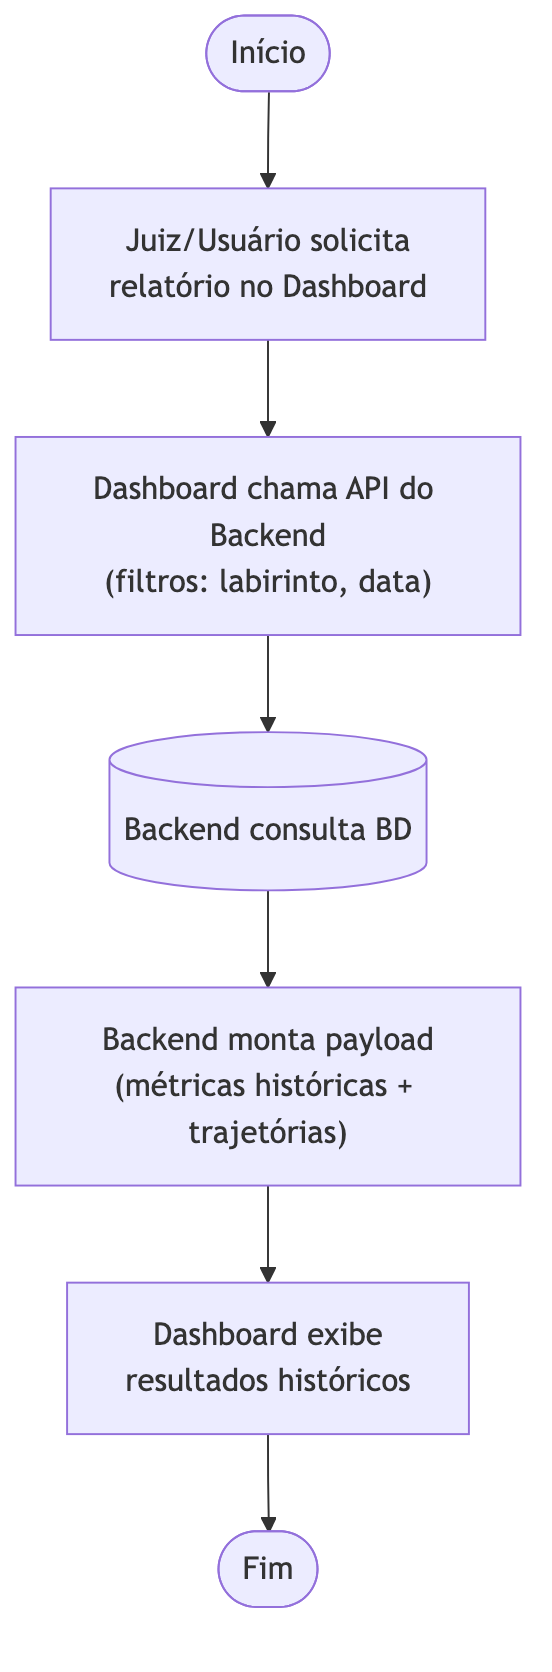
\includegraphics[width=0.85\linewidth,height=0.85\textheight,keepaspectratio]{figuras/diagrama_atividade_relatorio.png}
        \caption{Diagrama de atividades UML: fluxo de consulta a relatórios históricos.}
        \label{fig:diagrama_atividade_relatorio}
    \end{figure}

%=========================================================================================    
    \subsection{Backlog do Produto}

    Para identificar as principais necessidades do sistema, foram levantados os requisitos funcionais e não funcionais do micromouse, que descrevem tanto os comportamentos esperados quanto os critérios de qualidade e desempenho do sistema. Além disso, foi utilizada a técnica de priorização MoSCoW para classificar os requisitos de acordo com seu nível de importância para o desenvolvimento do projeto. Essa técnica organiza os requisitos em quatro categorias: Must Have, para requisitos essenciais; Should Have, para requisitos importantes; Could Have, para funcionalidades desejáveis; e Won’t Have, para funcionalidades que não serão implementadas na versão atual do projeto.
    
    A tabela abaixo apresenta os requisitos elicitados e suas respectivas classificações segundo a técnica MoSCoW.

    \begin{center}
    \begin{longtable}{|p{5.5cm}|p{8cm}|c|}
    \caption{Requisitos funcionais de navegação.} \label{tab:navegacao} \\
    \hline
    \textbf{Requisito} & \textbf{Descrição} & \textbf{MoSCoW} \\ \hline
    \endfirsthead
    \multicolumn{3}{c}{{\bfseries \tablename\ \thetable{} -- continuação da página anterior}} \\
    \hline
    \textbf{Requisito} & \textbf{Descrição} & \textbf{MoSCoW} \\ \hline
    \endhead
    \hline \multicolumn{3}{r}{{Continua na próxima página}} \\ \endfoot
    \hline \endlastfoot

    RF01 - \textbf{Mover-se para frente} & O micromouse deverá ser capaz de mover-se para frente durante a navegação no labirinto. & Must \\ \hline

    RF02 - \textbf{Rotacionar em até 180°} & O micromouse deverá ser capaz de realizar rotações de até 180° para alterar sua direção no labirinto. & Must \\ \hline

    RF03 - \textbf{Reconhecer paredes} & O sistema deverá ser capaz de reconhecer paredes ao redor do micromouse durante a navegação. & Must \\ \hline

    RF04 - \textbf{Medir distância até a parede} & O sistema deverá medir a distância entre o micromouse e as paredes do labirinto. & Must \\ \hline

    RF05 - \textbf{Identificar o caminho livre} & O micromouse deverá identificar caminhos livres disponíveis para navegação no labirinto. & Must \\ \hline

    RF06 - \textbf{Encontrar o caminho até o centro do labirinto} & O micromouse deverá encontrar o caminho até o centro do labirinto de forma autônoma. & Must \\ \hline

    RF07 - \textbf{Detectar a chegada ao objetivo do labirinto} & O sistema deverá detectar quando o micromouse alcançar o objetivo do labirinto. & Must \\ \hline

    RF08 - \textbf{Evitar colisões com as paredes} & O micromouse deverá evitar colisões com as paredes durante sua navegação. & Must \\ \hline

    RF09 - \textbf{Controlar os motores de locomoção do micromouse} & O sistema deverá controlar os motores responsáveis pela locomoção do micromouse. & Must \\ \hline

    RF10 - \textbf{Adquirir dados dos sensores de distância} & O sistema deverá adquirir dados dos sensores de distância utilizados pelo micromouse. & Must \\ \hline

    \end{longtable}
    \end{center}

    \begin{center}
    \begin{longtable}{|p{5.5cm}|p{8cm}|c|}
    \caption{Requisitos funcionais de telemetria.} \label{tab:telemetria} \\
    \hline
    \textbf{Requisito} & \textbf{Descrição} & \textbf{MoSCoW} \\ \hline
    \endfirsthead
    \multicolumn{3}{c}{{\bfseries \tablename\ \thetable{} -- continuação da página anterior}} \\
    \hline
    \textbf{Requisito} & \textbf{Descrição} & \textbf{MoSCoW} \\ \hline
    \endhead
    \hline \multicolumn{3}{r}{{Continua na próxima página}} \\ \endfoot
    \hline \endlastfoot

    RF11 - \textbf{Calcular velocidade média} & O sistema deverá calcular a velocidade média do micromouse durante a execução. & Must \\ \hline

    RF12 - \textbf{Calcular consumo de energia} & O sistema deverá calcular o consumo de energia do micromouse durante sua operação. & Must \\ \hline

    RF13 - \textbf{Salvar o caminho percorrido} & O sistema deverá salvar o trajeto percorrido pelo micromouse durante a navegação. & Must \\ \hline

    RF14 - \textbf{Mapear o labirinto} & O sistema deverá gerar um mapa do labirinto durante a execução. & Must \\ \hline

    RF15 - \textbf{Armazenar o mapa descoberto} & O sistema deverá armazenar o mapa descoberto pelo micromouse. & Must \\ \hline

    RF16 - \textbf{Exibir dados de telemetria em tempo real} & O sistema deverá exibir os dados de telemetria do micromouse em tempo real. & Must \\ \hline

    RF17 - \textbf{Enviar dados de telemetria em tempo real} & O micromouse deverá enviar os dados de telemetria em tempo real para o sistema web. & Must \\ \hline

    RF18 - \textbf{Monitorar o nível da bateria do sistema} & O sistema deverá monitorar o nível da bateria do micromouse. & Must \\ \hline

    RF19 - \textbf{Registrar o tempo total de operação do micromouse} & O sistema deverá registrar o tempo total de operação do micromouse. & Must \\ \hline

    RF20 - \textbf{Indicar o status de conclusão do desafio} & O sistema deverá indicar o status de conclusão do desafio após a execução do labirinto. & Must \\ \hline

    RF21 - \textbf{Monitorar a tensão da alimentação elétrica} & O sistema deverá monitorar a tensão da alimentação elétrica do micromouse. & Must \\ \hline

    RF22 - \textbf{Controlar remotamente a execução do micromouse} & O sistema deverá permitir iniciar e interromper remotamente a execução do micromouse. & Must \\ \hline

    \end{longtable}
    \end{center}

    \begin{center}
    \begin{longtable}{|p{5.5cm}|p{8cm}|c|}
    \caption{Requisitos não funcionais do micromouse.} \label{tab:rnf} \\
    \hline
    \textbf{Requisito} & \textbf{Descrição} & \textbf{MoSCoW} \\ \hline
    \endfirsthead
    \multicolumn{3}{c}{{\bfseries \tablename\ \thetable{} -- continuação da página anterior}} \\
    \hline
    \textbf{Requisito} & \textbf{Descrição} & \textbf{MoSCoW} \\ \hline
    \endhead
    \hline \multicolumn{3}{r}{{Continua na próxima página}} \\ \endfoot
    \hline \endlastfoot

    RNF01 - \textbf{Funcionamento autônomo} & O micromouse deverá funcionar de forma autônoma durante toda a execução do labirinto. & Must \\ \hline

    RNF02 - \textbf{Comunicação sem fio} & A comunicação entre o micromouse e o sistema de telemetria deverá ocorrer sem o uso de conexões cabeadas. & Must \\ \hline

    RNF03 - \textbf{Tempo de carregamento da telemetria} & A página de telemetria deverá carregar em até 5 segundos. & Must \\ \hline

    RNF04 - \textbf{Latência da telemetria} & A latência entre o envio e a exibição dos dados de telemetria deverá ser inferior a 1 segundo. & Must \\ \hline

    RNF05 - \textbf{Frequência de atualização} & O sistema deverá atualizar os dados de telemetria a cada 500 ms. & Must \\ \hline

    RNF06 - \textbf{Resistência a variações de iluminação} & O micromouse deverá continuar operando mesmo com variações de iluminação no ambiente. & Must \\ \hline

    RNF07 - \textbf{Precisão da medição} & O sistema deverá medir distâncias com precisão mínima de 1 cm. & Must \\ \hline

    RNF08 - \textbf{Autonomia energética} & O micromouse deverá possuir autonomia suficiente para concluir o labirinto em menos de 30 minutos. & Should \\ \hline

    RNF09 - \textbf{Dimensões máximas} & O micromouse deverá possuir dimensões inferiores a 18 cm × 18 cm. & Must \\ \hline

    RNF10 - \textbf{Estabilidade elétrica} & O sistema deverá operar sem reinicializações causadas por oscilações de tensão durante a execução do labirinto. & Must \\ \hline

    RNF11 - \textbf{Resistência a colisões} & O micromouse deverá continuar operacional após 10 colisões leves consecutivas. & Should \\ \hline

    \end{longtable}
    \end{center}

    \subsection{Histórias de Usuário}
      As histórias de usuário foram definidas a partir dos requisitos funcionais e não funcionais levantados para o sistema. Todas as histórias foram documentadas juntamente com seus respectivos critérios de avaliação no repositório do GitHub do projeto. Além disso, a equipe desenvolveu um protótipo para as histórias relacionadas aos requisitos de telemetria, o qual pode ser visualizado nas respectivas issues de telemetria do repositório.
    \begin{center}

    \begin{multicols}{2}
    \begin{itemize}
        \item HU01 -- Movimentação frontal
        \item HU02 -- Rotação do micromouse
        \item HU03 -- Reconhecimento de paredes
        \item HU04 -- Medição de distância
        \item HU05 -- Identificação de caminhos livres
        \item HU06 -- Navegação até o objetivo
        \item HU07 -- Detecção de chegada ao objetivo
        \item HU08 -- Prevenção de colisões
        \item HU09 -- Cálculo de velocidade média
        \item HU10 -- Cálculo de consumo energético
        \item HU11 -- Salvamento do caminho percorrido
        \item HU12 -- Mapeamento do labirinto
        \item HU13 -- Armazenamento do mapa
        \item HU14 -- Exibição de telemetria
        \item HU15 -- Envio de telemetria
        \item HU16 -- Monitoramento da bateria
        \item HU17 -- Registro de tempo de operação
        \item HU18 -- Indicação de conclusão do desafio
        \item HU19 -- Controle dos motores
        \item HU20 -- Aquisição de dados dos sensores
        \item HU21 -- Monitoramento da alimentação elétrica
        \item HU22 -- Controle remoto da execução
    \end{itemize}
    \end{multicols}        
    \end{center}




%=========================================================================================    
    \subsection{Arquitetura de Software}

    O software embarcado permitirá que o robô Micromouse percorra autonomamente um labirinto modular 4x4 e 8x8, sensoriando as paredes, atualizando um mapa interno, decidindo o próximo movimento por flood-fill e executando o deslocamento por controle de motores. Os serviços de apoio, compostos por backend e dashboard, permitirão operação supervisionada, exibindo trajetória, leituras e estado interno do sistema em tempo real.

    A arquitetura é distribuída em quatro componentes, integrados por um message broker, com o objetivo de desacoplar o robô (produtor) do backend (consumidor):
    \begin{itemize}
        \item \textbf{Nó embarcado}: firmware no Raspberry Pi Pico W (RP2040 dual-core), responsável pelas malhas de tempo crítico -- sensoriamento, navegação, controle de motores e publicação de telemetria.
        \item \textbf{Broker MQTT} (Mosquitto): media a comunicação assíncrona entre robô e backend, com entrega QoS 1 e retenção de mensagens de estado.
        \item \textbf{Backend}: serviço HTTP que assina os tópicos MQTT, persiste os dados de execução, expõe API REST para consultas históricas e propaga atualizações ao dashboard por canal push.
        \item \textbf{Frontend}: single-page application de dashboard, voltada à operação supervisionada e à análise dos dados do robô.
    \end{itemize}

    Essa separação se justifica porque o microcontrolador não possui recursos para servir interfaces web, porque os requisitos de tempo crítico do controle dos motores inviabilizam o acoplamento da malha de controle a operações de rede, e porque o broker MQTT fornece entrega garantida com QoS 1, persistência de estado por mensagens retained e suporte nativo a múltiplos consumidores -- um padrão consolidado em aplicações IoT.

    \textbf{Stack tecnológica:}
    \begin{itemize}
        \item \textbf{Firmware}: C++17 com Pico SDK; drivers de baixo nível em C, consumidos como cabeçalhos pelo firmware em C++.
        \item \textbf{Broker}: Eclipse Mosquitto em container Docker.
        \item \textbf{Backend}: Python com Django, Django REST Framework, Celery com Redis (worker subscriber MQTT), httpx e gerenciamento por uv; autenticação JWT; PostgreSQL, aproveitando UUID v7.
        \item \textbf{Frontend}: TypeScript com React, Vite, Mantine, TanStack Query, React Router e gerenciamento por pnpm.
    \end{itemize}

    A descrição da arquitetura segue o modelo 4+1 de Kruchten, a partir das visões lógica, de processos, de implementação, de implantação e de dados.

    \textbf{Visão lógica.} O sensoriamento abstrai os sensores HC-SR04, VL53L0X e MPU-6050, fornecendo distâncias de parede e orientação angular tratada. A localização mantém a posição do robô em coordenadas de célula e orientação cardinal, atualizadas por odometria dos encoders e corrigidas pela IMU. O mapeamento representa o labirinto como matriz 4x4 ou 8x8, com quatro flags de parede por célula. O planejamento, baseado em flood-fill, calcula o próximo movimento tendo a célula central como objetivo. O controle de movimento converte o alvo em PWM para o driver TB6612FNG, fechando a malha sobre os encoders dos motores N20 (estratégia de controle e ganhos ainda a calibrar). A comunicação embarcada publica o estado do robô via MQTT em tópicos por identificador de robô; a matriz delta já calculada é enviada, evitando duplicar lógica entre firmware e backend. No backend, um worker assina os tópicos MQTT, processa as mensagens por use cases, persiste os dados no PostgreSQL, expõe API REST e fornece canal WebSocket ao frontend, que visualiza labirinto, posição, trajetória e controles de operação.

    \textbf{Visão de processos.} No RP2040, o Core 1 será dedicado às tarefas de tempo real -- aquisição de sensores, algoritmo flood-fill e controle dos motores --, isolando o controle das latências do scheduler. O Core 0 executará a stack Wi-Fi, o cliente MQTT e a telemetria, isolando o caminho crítico das latências de rede. Para evitar contenção no barramento I2C, apenas a tarefa de aquisição lerá os sensores, publicando em um buffer compartilhado consumido independentemente pelo algoritmo e pela telemetria. As frequências de amostragem dos sensores e de controle são estimativas iniciais, sujeitas a calibração durante a implementação. No backend cooperam três processos: o web server, servindo a API REST; o worker que assina os tópicos MQTT e dispara os use cases de persistência e propagação; e o canal push ao dashboard (WebSocket ou SSE, a confirmar). No frontend, a SPA usa TanStack Query para estado de servidor, Mantine para a interface e um canal push para telemetria.

    \textbf{Visão de implementação.} Propõe-se um monorepo com os diretórios de firmware, backend e frontend. O firmware será organizado por responsabilidade -- inicialização, sensoriamento, localização, planejamento, controle de motores, comunicação e drivers. O backend será uma aplicação Django com DRF e Celery, organizada em um app de infraestrutura (base de modelos, erros e autenticação), um app de integrações (MQTT e storage) e o app de domínio principal, reunindo modelos, use cases, API REST e testes. O frontend, em Vite/React/Mantine, seguirá organização por domínio, com componentes de visualização do labirinto e hooks de consumo da telemetria em tempo real. A subequipe de Eletrônica entregará os drivers em C, consumidos pelo firmware em C++ -- principal ponto de delegação entre as subequipes.

    \textbf{Visão de implantação.} Quatro nós físicos compõem o sistema. O nó embarcado (Pico W) comunica-se com os periféricos por barramentos digitais -- HC-SR04 (trigger/echo via GPIO), VL53L0X (I2C, endereço 0x29), MPU-6050 (I2C, endereços 0x68 ou 0x69, mesmo barramento), TB6612FNG (GPIO/PWM) e encoders (interrupções GPIO) -- e publica telemetria via Wi-Fi. O nó de broker roda Mosquitto em container Docker, no mesmo host do backend durante desenvolvimento e competição. O nó de serviços executa o backend, o worker Celery, Redis e PostgreSQL, empacotados em Docker Compose; o deploy em ambiente de produção dedicado ainda está a confirmar. O nó de apresentação é o navegador do operador, conectado ao backend via API REST e canal push. Os tópicos MQTT são: telemetria (posição, velocidade e bateria, QoS 1), evento (início, colisão, reparo, desafio cumprido, QoS 1 retained) e status (heartbeat online/offline via Last Will and Testament, QoS 1 retained). A pinagem do Pico W e o detalhamento elétrico estão na Seção 6.3, do Capítulo 6.

    \textbf{Visão de dados.} A persistência ocorre em PostgreSQL. Todas as entidades herdam de uma classe base com chave primária UUID v7, ordenável temporalmente, e campos de criação/atualização automáticos. As migrations seguem o padrão Django, com prefixo numérico.


\subsection{Modelo Entidade-Relacionamento (MER)}

\textbf{Entidades:}

\begin{itemize}
    \item MICROMOUSE
    \item LABIRINTO
    \item TENTATIVA
    \item POSICAO
\end{itemize}

\vspace{0.5cm}

\textbf{Atributos:}

\begin{itemize}
    \item \textbf{MICROMOUSE} (\underline{id}, nome, algoritmo)

    \item \textbf{LABIRINTO} (\underline{id}, nome, dimensao)

    \item \textbf{TENTATIVA} (\underline{id}, tempo\_inicio, tempo\_fim, consumo\_bateria, velocidade\_media, sucesso, micromouse\_id, labirinto\_id)

    \item \textbf{POSICAO} (\underline{id}, coordenada\_x, coordenada\_y, timestamp, passo, tentativa\_id)
\end{itemize}

\vspace{0.5cm}

\textbf{Relacionamentos:}

\begin{itemize}
    \item \textbf{REALIZA}
    \begin{itemize}
        \item MICROMOUSE (1:N) TENTATIVA
    \end{itemize}

    \item \textbf{USA}
    \begin{itemize}
        \item LABIRINTO (1:N) TENTATIVA
    \end{itemize}

    \item \textbf{POSSUI}
    \begin{itemize}
        \item TENTATIVA (1:N) POSICAO
    \end{itemize}
\end{itemize}

\vspace{0.3cm}

    \subsection{Diagrama Entidade-Relacionamento (DER)}
            
        \begin{figure}[H]
            \centering
            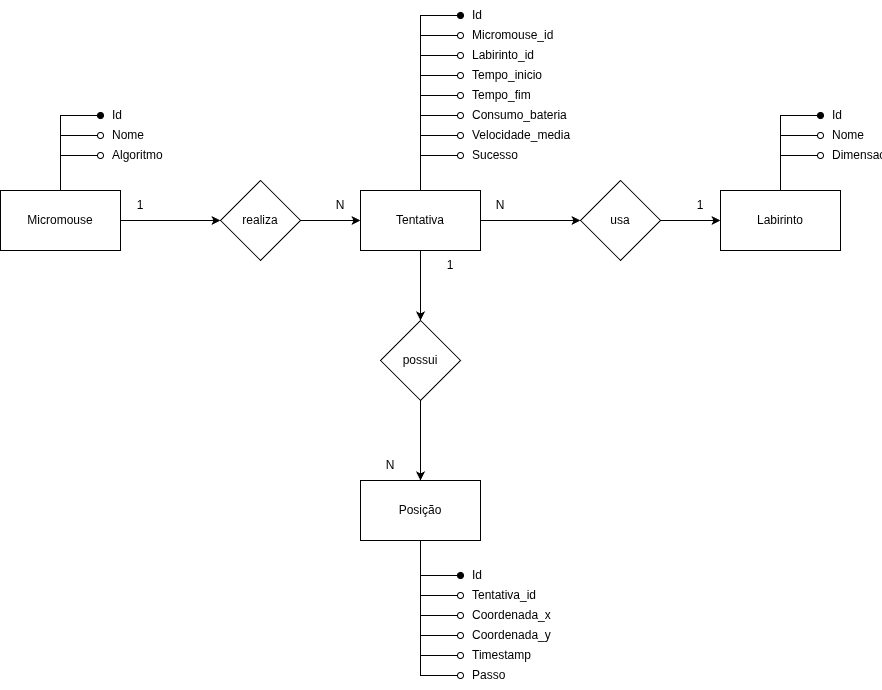
\includegraphics[width=0.8\textwidth]{../../docs/img/Diagrama_entidades.png}
            \caption{Diagrama Entidade-Relacionamento}
            \label{fig:diagrama_entidades}
        \end{figure}
        
%    \item \textcolor{red}{\textbf{ Roteiro de testes funcionais:} }
%    \begin{itemize}
%        \item \textcolor{red}{Código do caso de teste;}
%        \item \textcolor{red}{Nome do caso de teste;}
%        \item \textcolor{red}{ Objetivo do caso de teste;}
%        \item \textcolor{red}{ Pré-condições do sistema para o teste ser realizado, quando se aplicar;}
%        \item \textcolor{red}{ Descrição dos procedimentos a serem executados para o teste;}
%        \item \textcolor{red}{ Resultado esperado para o teste ser aprovado (pós-condição após realizado o teste);}
%    \end{itemize}
%\end{itemize}

%=========================================================================================
\subsection{Detalhamento dos Casos de Teste}

Abaixo estão alguns dos casos de testes que serão feitos para verificação e validação do desenvolvimento do micromouse. O link mostra todos os casos de testes com as suas caraterísticas e especificações mostradas na GitPages.

GitPages: \url{https://fcte-pi1.github.io/2026_1_PI1_Grupo02_Juliana/software/casosteste/}

    \subsubsection{CT01 - Validação do Sistema Sensorial e Precisão}
    \begin{itemize}
        \item \textbf{Nome do caso de teste:} CT01 - Leitura e Calibração dos Sensores de Distância (RF03, RF04, RF10, RNF07).
        \item \textbf{Objetivo do caso de teste:} Validar se o sistema reconhece as paredes, adquire os dados corretamente e mede a distância com a precisão mínima exigida.
        \item \textbf{Pré-condições:} Micromouse montado e posicionado em uma célula de teste; monitor serial ou telemetria ativos.
        \item \textbf{Descrição dos procedimentos:}
        \begin{enumerate}
            \item Posicionar o robô a distâncias 6cm, 12cm, 18cm(que corresponde ao tamanho de uma célula) de uma parede.
            \item Registrar o valor reportado pelo sistema para cada sensor.
            \item Verificar se o software identifica a presença de parede quando a distância for inferior ao limite da célula.
        \end{enumerate}
        \item \textbf{Resultado esperado:} O erro de medição deve ser inferior a 1 cm, conforme o requisito RNF07. O sistema deve sinalizar corretamente a existência de obstruções à frente e nas laterais.
    \end{itemize}

    \subsubsection{CT02 - Controle de Trajetória e Estabilidade Elétrica}
    \begin{itemize}
        \item \textbf{Nome do caso de teste:} CT02 - Deslocamento Retilíneo e Controle de Motores (RF01, RF08, RF09, RNF10).
        \item \textbf{Objetivo do caso de teste:} Validar a capacidade de mover-se para frente controlando os motores para evitar colisões sem reinicializações elétricas.
        \item \textbf{Pré-condições:} Bateria carregada; corredor reto livre de obstáculos imprevistos.
        \item \textbf{Descrição dos procedimentos:}
        \begin{enumerate}
            \item Acionar o comando de avanço para percorrer três células consecutivas.
            \item Observar se o robô mantém a trajetória centralizada usando o controle dos motores.
            \item Monitorar se ocorrem quedas de tensão que causem o reset do microcontrolador.
        \end{enumerate}
        \item \textbf{Resultado esperado:} O robô deve completar o percurso sem tocar nas paredes laterais e o sistema deve permanecer estável, sem oscilações de tensão que interrompam a execução.
    \end{itemize}

    \subsubsection{CT03 - Precisão de Manobra e Alteração de Direção}
    \begin{itemize}
        \item \textbf{Nome do caso de teste:} CT03 - Rotação e Mudança de Orientação (RF02, RF09).
        \item \textbf{Objetivo do caso de teste:} Garantir que o micromouse realize rotações de até 180° através do controle preciso dos motores.
        \item \textbf{Pré-condições:} Robô parado no centro de uma célula.
        \item \textbf{Descrição dos procedimentos:}
        \begin{enumerate}
            \item Comandar uma rotação de 90° para a esquerda e medir o ângulo final.
            \item Comandar uma rotação de 90° para a direita e medir o ângulo final.
            \item Comandar uma rotação de 180° (meia-volta).
        \end{enumerate}
        \item \textbf{Resultado esperado:} O robô deve realizar as rotações solicitadas com erro angular mínimo, permitindo que ele continue a navegação alinhado ao novo corredor.
    \end{itemize}

    \subsubsection{CT04 - Inteligência e Navegação Autônoma}
    \begin{itemize}
        \item \textbf{Nome do caso de teste:} CT04 - Mapeamento e Busca do Centro (RF05, RF06, RF07, RF14, RNF01).
        \item \textbf{Objetivo do caso de teste:} Validar o funcionamento autônomo na identificação de caminhos, geração do mapa e alcance do objetivo central.
        \item \textbf{Pré-condições:} Labirinto desconhecido pelo robô; algoritmo de navegação (ex: Flood Fill) carregado.
        \item \textbf{Descrição dos procedimentos:}
        \begin{enumerate}
            \item Iniciar o robô na célula inicial (0,0) em modo autônomo.
            \item Observar se o robô identifica caminhos livres e mapeia as paredes encontradas.
            \item Verificar se o sistema detecta a chegada ao objetivo central do labirinto.
        \end{enumerate}
        \item \textbf{Resultado esperado:} O micromouse deve encontrar o caminho até o centro de forma autônoma e o mapa gerado internamente deve corresponder à realidade física do labirinto.
    \end{itemize}

    \subsubsection{CT05 - Telemetria e Comunicação sem Fio}
    \begin{itemize}
        \item \textbf{Nome do caso de teste:} CT05 - Validação de Telemetria em Tempo Real (RF16, RF17, RNF04).
        \item \textbf{Objetivo:} Verificar se os dados de navegação são enviados e exibidos na interface web com a latência exigida.
        \item \textbf{Pré-condições:} Micromouse conectado à rede sem fio; sistema web de telemetria ativo e aguardando conexão.
        \item \textbf{Descrição dos procedimentos:}
        \begin{enumerate}
            \item Iniciar a movimentação do robô no labirinto.
            \item Observar a atualização dos campos de velocidade e posição na interface web.
            \item Cronometrar o tempo entre um evento físico (ex: detecção de parede) e sua exibição na tela.
        \end{enumerate}
        \item \textbf{Resultado esperado:} Os dados devem ser atualizados a cada 500 ms (RNF05) com latência inferior a 1 segundo (RNF04). A interface deve exibir corretamente a posição X e Y enviada pelo robô.
    \end{itemize}

    
% \textcolor{red}{Com relação ao \textit{software}, será necessário apresentar os seguintes itens: % pacotes de componentes de \textit{software}, suas funções e características, e explicar as decisões de projeto:
% \begin{enumerate}
%     \item Um diagrama do processo de negócio do problema que a máquina se propõe a resolver (BPNM) – não é UML, mas é fundamental para entender como o sistema se comporta como um todo, incluindo o usuário;
%     \item Lista de casos de uso (backlog do sistema). Backlog funcional;
%     \item Lista de requisitos não-funcionais a serem satisfeitos pelo sistema;
%     \item Diagrama de casos de uso: mostrando os requisitos funcionais, seus atores e como eles interagem entre si;
%     \item Diagrama de Classes: apresentando quais dados são manipulados pelo sistema (internamente e externamente – ex.: resultados de experimentos);
%     \item Diagrama de arquitetura, identificando todos os componentes da máquina e suas iterações com o software;
%     \item Diagrama de estados da máquina (sistema);
%     \item Descrição dos testes dos componentes da máquina e dos testes funcionais que deveriam ser feitos para avaliar o funcionamento da máquina e identificar defeitos. São importantes os testes unitários (componentes) e de integração (conjunto de componentes) e o roteiro de testes.
% \end{enumerate}
% }
%\textcolor{red}{Com relação ao \textit{software}, será necessário apresentar pacotes de componentes de \textit{software}, suas funções e características, e explicar as decisões de projeto.}
